\section{Gluon emission from a parent quark}
\label{fir}
\begin{figure}[ht!]
\centering
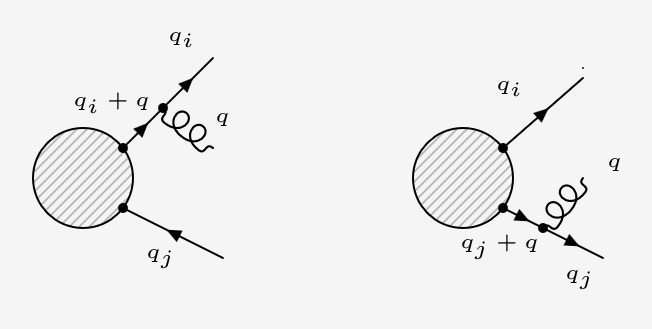
\includegraphics[width=0.85\textwidth]{images/QQ/qqg-diagrams.png}
\label{qg}
\end{figure}
First of all contemplate a quark gluon splitting with an arbitrary spectator like an anti-quark with the momentum $ q_j $. Where $ q_j+q $ is the momentum of the parent quark before splitting, $q$ the momentum of the gluon and $q_i$ of the daughter quark respectively. The distinction between daughter and parent vanishes, when the gluon becomes soft,  and a
singularity develops. The other possibility to get a singularity is when the gluon is collinear to the (anti)-quark. The splitting functions are flavour independent since the strong interaction is flavour independent. Furthermore, leading order splitting cannot change the flavour of a quark, thus \cite{halzen1984quarks}:
\begin{equation}
\begin{split}
P_{{\bar{q_i}}{\bar{q_j}}}=P_{{q_i}{q_j}}\equiv P_{{q}{q}} \delta_{ij}\\
P_{{\bar{q_i}}{{g}}}=P_{{q_i}{g}}\equiv P_{{q}{g}} \\
P_{{\bar{g}}{\bar{q_i}}}=P_{{g}{q_i}}\equiv P_{{g}{q}} \delta_{ij}\\
\end{split}
\end{equation}
%Since there is no distinction between quark and anti-quark, one can imagine exact the same splitting variation for anti-quark.


\pagebreak
\subsection{Matrix element of a quark with a gluon radiation $ |M_1|^2 $}

\begin{figure}[h!]
\centering
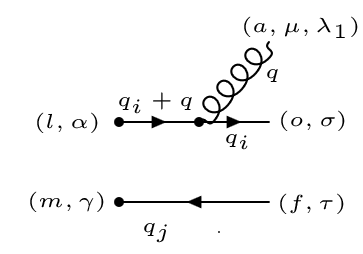
\includegraphics[scale=0.7]{images/QQ/qgqbarM.png}
\end{figure}
The first step of the procedure is to label the diagrams independently and use the Feynman rules:
\begin{equation}
M_1 = [{\bar{u}}_{\sigma}(q_i) (-ig_s \gamma^{\mu}\times {[T^a]_o}^l)  \frac{i(\not{q_i} + \not{q})}{(q_i + q)^2} {\varepsilon^{\lambda_1}}_{\mu} (q)]\: [{v}_{\tau}(q_j)]
\end{equation}
For the quadratic matrix element the hermitian conjugate of $ M_1 $ needs to be calculated.
\begin{figure}[h!]
\centering
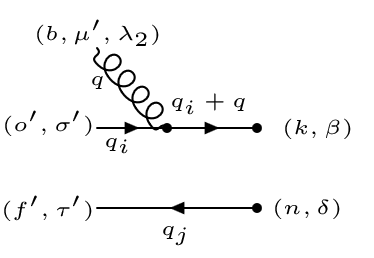
\includegraphics[scale=0.7]{images/QQ/qgqbarMDega.png}
\end{figure}

\begin{equation}
{M_1}^{\dagger} = [\frac{-i(\not{q_i} + \not{q})}{(q_i + q)^2} \:  (ig_s \gamma^{{\mu}^{\prime}}\times {[T^b]_{o\:^{\prime}}}^k) \: u_{{\sigma}^{\prime}}(q_i) \: {\varepsilon^{\lambda_2}}_{{\mu}^{\prime}} (q)][{\bar{v}}_{{\tau}^{\prime}}(q_j)]
\end{equation}
\pagebreak
\begin{figure}[h!]
\centering
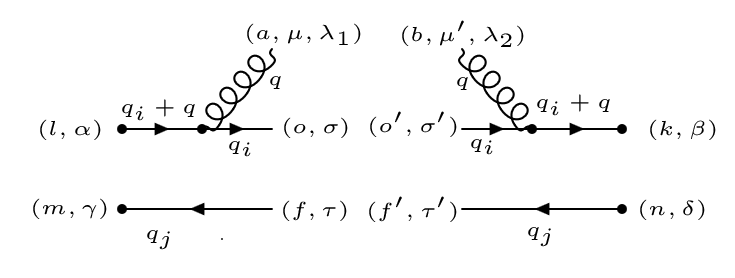
\includegraphics[width=0.85\textwidth]{images/QQ/qgqbarMSquer.png}
\end{figure}
Multiplying $ {M_1}^{\dagger} $ and $ {M_1} $ and putting the diagrams next to each other:
\begin{equation}
\begin{split}
|M_1|^2=M_1\:{\color[RGB]{255,0,0} {M_1}^{\dagger}} = [{\bar{u}}_{\sigma}(q_i)\: (-ig_s \gamma^{\mu}\times {[T^a]_o}^l) \: \frac{i(\not{q_i} + \not{q})}{(q_i + q)^2}\:\: {\varepsilon^{\lambda_1}}_{\mu} (q)] [{v}_{\tau}(q_j)]\: \\
\quad\quad\quad\quad\quad\quad\quad\quad\:\:{\color[RGB]{255,0,0}[\frac{-i(\not{q_i} + \not{q})}{(q_i + q)^2} \:  (ig_s \gamma^{{\mu}^{\prime}}\times {[T^b]_{o\:^{\prime}}}^k) \: u_{{\sigma}^{\prime}}(q_i) \: {{\varepsilon^{\lambda_2}}_{{\mu}^{\prime}}}^* (q)][{\bar{v}}_{{\tau}^{\prime}}(q_j)]}
\end{split}
\end{equation}
Connecting those terms which are related to each other:

\begin{equation}
\begin{split}
|M_1|^2=[\frac{-i(\not{q_i} + \not{q})}{(q_i + q)^2} \:
 \:  (ig_s \gamma^{{\mu}^{\prime}}\times {[T^b]_{o\:^{\prime}}}^k) \: {\bar{u}}_{\sigma}(q_i)\:u_{{\sigma}^{\prime}}(q_i) \: {{\varepsilon^{\lambda_2}}_{{\mu}^{\prime}}^* (q) {\varepsilon^{\lambda_1}}_{\mu} (q)} \\
\times (-ig_s \gamma^{\mu}\times {[T^a]_o}^l) \: \frac{i(\not{q_i} + \not{q})}{(q_i + q)^2} ]
[{\bar{v}}_{{\tau}^{\prime}}(q_j) {v}_{\tau}(q_j)]
\end{split}
\end{equation}

Sum over the lorenz index $({\sigma},{\sigma}^{\prime})$ and $({\tau},{\tau}^{\prime})$ and spin addition relation for massless quarks leads to:
 
\begin{equation}
\begin{split}
\displaystyle\sum\limits_{{\sigma},{\sigma}^{\prime}} {\bar{u}}_{\sigma}(q_i)\:u_{{\sigma}^{\prime}}(q_i) = \not{q_i},\\
\displaystyle\sum\limits_{{\tau},{\tau}^{\prime}} {\bar{v}}_{\tau}(q_j)\:v_{{\tau}^{\prime}}(q_j) = \not{q_j} 
\end{split}
\end{equation}
According to the equation \ref{Feynman} in Feynman gauge ($ \zeta \rightarrow 1 $), the sum over polarization index $({\lambda_{1}},{\lambda}_{2})$ for massless Gluons will be:
\begin{equation}
\begin{split}
 \displaystyle\sum\limits_{{\mu},{\mu}^{\prime}} {{\varepsilon^{\lambda_2}}_{{\mu}^{\prime}}^* (q) {\varepsilon^{\lambda_1}}_{\mu} (q)} = -g_{{\mu}{\mu}^{\prime}} 
\end{split}
\end{equation}
The matrix element will be simplified with: 
\begin{equation}
\begin{split}
|M_1|^2=\frac{-g_s^2  {[T^a]_{o}}^k \: {[T^a]_o}^l }{(q_i + q)^2 (q_i + q)^2}
[(\not{q_i} + \not{q}) \:
 \:  \gamma^{{\mu}^{\prime}} \: \not{q_i} \: g_{{{\mu}^{\prime}}{\mu}} 
\gamma^{\mu} \: (\not{q_i} + q)]
[\not{q_j}]
\end{split}
\end{equation}

As it was discussed in the procedure the contracted indices lead us to the predict the relevant singular terms:
\begin{equation}
\begin{split}
|M_1|^2=\frac{-g_s^2  {[T^a]_{o}}^k \: {[T^a]_o}^l }{(q_i + q)^2 (q_i + q)^2}
[(\not{q_i} + \not{q}) \:
 \:  \gamma^{{\mu}^{\prime}} \: \not{q_i} \: 
\gamma_{{\mu}^{\prime}} \: (\not{q_i} + q)]
[\not{q_j}]
\label{first}
\end{split}
\end{equation}

From the result the tree level diagram from LO and a number are expected:\\
\begin{figure}[h!]
\centering
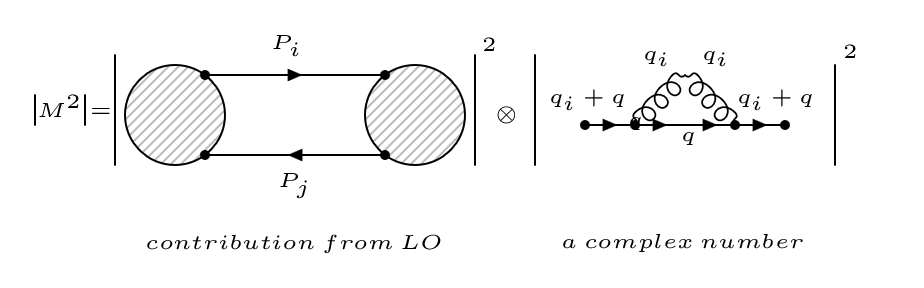
\includegraphics[width=0.85\textwidth]{images/QQ/expectationqg-qbar.png}
\end{figure}
Which graphically means:\\
\begin{equation}
\begin{split}
|M_1|^2=\frac{-g_s^2  {[T^a]_{o}}^k \: {[T^a]_o}^l }{(q_i + q)^2 (q_i + q)^2}
[\not{P_i}]
[\not{P_j}]\:\times \: {\color[RGB]{255,0,0} (a\: complex\: number)}
\end{split}
\end{equation}  
Let's calculate the contribution and compare the final result with this expectation. Calculating the expression in the parentheses from the equation \ref{first} separately results in:
\begin{equation}
\begin{split}
N=&: \gamma^{{\mu}^{\prime}} \not{q_i} \: \gamma_{{\mu}^{\prime}} = {q_{i\sigma}} \: \gamma^{{\mu}^{\prime}} \gamma^{\sigma} \:\: \gamma_{{\mu}^{\prime}}\\
=& \: {q_{i\sigma}} \: (\lbrace{\gamma^{{\mu}^{\prime}}}, {\gamma^{\sigma}}\rbrace \: - {\gamma^{\sigma}}{\gamma^{{\mu}^{\prime}}})\gamma_{{\mu}^{\prime}}\\
=& \:{q_{i\sigma}} \: 2g^{{{\mu}^{\prime}}{\sigma}} \: \gamma_{{\mu}^{\prime}} \: - \:d\:{\gamma^{\sigma}}\\
=& \:(2-d) \not{q_i}
\end{split}
\end{equation}
Simplification of the bracket:
\begin{equation}
\begin{split}
|M_1|^2=-(2-d)\:\frac{g_s^2  {[T^a]_{o}}^k \: {[T^a]_o}^l }{(q_i + q)^2 (q_i + q)^2}
[(\not{q_i} + \not{q}) \:
 \:\not{q_i} \: 
 \: (\not{q_i} + q)]
[\not{q_j}]
\end{split}
\end{equation}

\begin{equation}
\begin{split}
|M_1|^2=-(2-d)\:\frac{g_s^2  {[T^a]_{o}}^k \: {[T^a]_o}^l }{(q_i + q)^2 (q_i + q)^2}
[\not{q_i} \not{q_i} \not{q_i} \: + \: \not{q_i} \not{q_i} \not{q} \: + \: \not{q} \not{q_i} \not{q_i} \:+\: \not{q} \not{q_i} \not{q}]
[\not{q_j}]
\end{split}
\end{equation}

With on-shell condition:
\begin{equation}
\begin{split}
\not{q_i}\: \not{q_i} &= {q_i}^2= {m_i}^2\\
\not{q} \: \not{q} &= {q}^2= {m}^2\\
\not{q_j}\not{q_j} &= {q_j}^2= {m_j}^2
\end{split}
\end{equation}

In terms of massless partons:

\begin{equation}
\begin{split}
|M_1|^2=-(2-d)\:\frac{g_s^2  {[T^a]_{o}}^k \: {[T^a]_o}^l }{(2q_i q)(2q_i q)}
[\not{q} \not{q_i} \not{q}]
[\not{q_j}]
\end{split}
\end{equation}
The terms in the brackets can be simplified:
\begin{equation}
\begin{split}
L=& \not{q} \not{q_i} \not{q} =\not{q}[{q_{i\sigma}} q_{\mu} \: (\lbrace{\gamma^{\mu}}, {\gamma^{\sigma}}\rbrace - {\gamma^{\sigma}}{\gamma^{\mu}})]\\ 
=& \not{q}[2{q_{i}}^{\mu} q_{\mu} - {q_{i\sigma}}q_{\mu}{\gamma^{\mu}}{\gamma^{\sigma}}\\
=& \not{q} (2q_i q)-q_{\mu}{q_{i\sigma}}q_{\mu}[{\gamma^{\mu}}{\gamma^{\mu}}{\gamma^{\sigma}}]\\
=& \not{q} (2q_i q)-q_{\mu}{q_{i\sigma}}q_{\mu}[\frac{{\gamma^{\mu}}{\gamma^{\mu}}}{2} +\frac{{\gamma^{\mu}}{\gamma^{\mu}}}{2}]{\gamma^{\sigma}}\\
=& \not{q} (2q_i q)-q_{\mu}{q_{i\sigma}}q_{\mu}[g^{{\mu}{\mu}}]{\gamma^{\sigma}}\\
=& \not{q} (2q_i q)-q_{\mu}{q_{i\sigma}}q^{\mu}{\gamma^{\sigma}}
=\not{q} (2q_i q)-q^2 \not{q_i}\\
=& \not{q} (2q_i q)
\end{split}
\end{equation}
After inserting the last result of $ L $ and simplify the term $ (2q_i q) $ from the denominator and nominator, the result becomes:
\begin{equation}
\begin{split}
|M_1|^2=-(2-d)\:\frac{g_s^2  {[T^a]_{o}}^k \: {[T^a]_o}^l }{2y(p_i \cdot p_j)}
[\not{q}]
[\not{q_j}]
\end{split}
\end{equation}
Now the old parametrisation will be used from equation \ref{par} to reduce the $ 3 $-partons matrix element to $ 2 $-partons:
\begin{equation}
\begin{split}
|M_1|^2=(d-2)\:\frac{g_s^2  {[T^a]_{o}}^k \: {[T^a]_o}^l }{2y(p_i \cdot p_j)}
[(1-z) \not{p_i}+zy \not{p_j} - \sqrt{zy(1-z)} \not{{m}_{\bot}}]
[(1-y) \not{p_j}]
\end{split}
\end{equation}
Multiplying the both sides 
\begin{equation}
\begin{split}
|M_1|^2=(d-2)\:\frac{g_s^2  {[T^a]_{o}}^k \: {[T^a]_o}^l }{2y(p_i \cdot p_j)}
[(1-z)(1-y) \not{p_i}\not{p_j} \\
+zy(1-y) \not{p_j}\not{p_j} - (1-y)\sqrt{zy(1-z)} \not{{m}_{\bot}}\not{p_j}]
\end{split}
\end{equation}
Under consideration of the fact that $ p_i $ and $ p_j $ are the on-shell momenta of the emitter and spectator partons, the terms with $ \not{p_i} \not{p_i} $ and $ \not{p_j} \not{p_j} $ can be eliminated.
The $ {p_i} \cdot  {m}_{\bot} $ and $ {p_j} \cdot  {m}_{\bot} $ are always $ 0 $ because the $ p_i $ and $ p_j $ are light like, i.e. zero transverse component. So those terms can be neglected.


\begin{equation}
\begin{split}
|M_1|^2=\frac{g_s^2  {[T^a]_{o}}^k \: {[T^a]_o}^l }{2y(p_i \cdot p_j)}
[\not{p_i}][\not{p_j}]\times(d-2)(1-z)(1-y)
\end{split}
\end{equation}

Expected was a contribution result from the LO and a complex number. The number is just for $ y \rightarrow 0 $ singular and not for $ z \rightarrow 1 $.

\newpage

\subsection{Matrix element of an anti-quark with a gluon radiation $ |M_2|^2 $}

%\begin{figure}[h!]
%\centering
%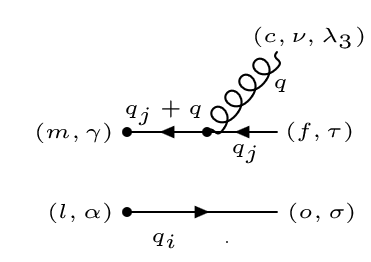
\includegraphics[scale=0.7]{images/QQ/qbargqM.png}
%\end{figure}
%
%\begin{equation}
%M_2 = [\frac{i(\not{q_j} + \not{q})}{(q_j + q)^2} (-ig_s \gamma^{\nu}\times {[T^c]_f}^m) \:{v}_{\tau}(q_j)\: {\varepsilon^{\lambda_3}}_{\nu} (q)]\: [{u}_{\sigma}(q_i)]
%\end{equation}
%\begin{figure}[h!]
%\centering
%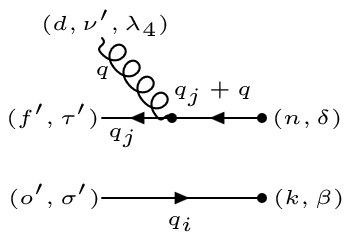
\includegraphics[scale=0.7]{images/QQ/qbargqMDega.png}
%\end{figure}
%\begin{equation}
%M_2^{\dagger} = [\bar{v}_{{\tau}^{\prime}}(q_j) \: (ig_s \gamma^{{\nu}^{\prime}}\times {[T^d]_{f^{\prime}}}^n) \: \frac{-i(\not{q_j} + \not{q})}{(q_j + q)^2} \: {\varepsilon^{\lambda_4}}_{{\nu}^{\prime}} (q)]\: [\bar{u}_{{\sigma}^{\prime}}(q_i)]
%\end{equation}
The same procedure is used to obtain the matrix element for an anti-quark with a single gluon emission.
\begin{figure}[h!]
\centering
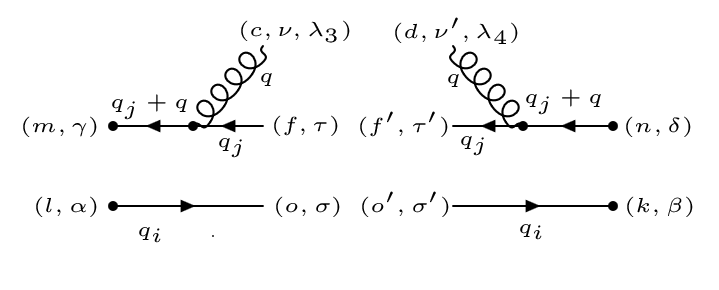
\includegraphics[width=0.85\textwidth]{images/QQ/qbargqMSquer.png}
\end{figure}

\begin{equation}
\begin{split}
|M_2|^2=M_2\:{\color[RGB]{255,0,0} {M_2}^{\dagger}} = [\frac{i(\not{q_j} + \not{q})}{(q_j + q)^2} (-ig_s \gamma^{\nu}\times {[T^c]_f}^m) \:{v}_{\tau}(q_j)\: {\varepsilon^{\lambda_3}}_{\nu} (q)]\: [{u}_{\sigma}(q_i)]\: \\
\quad\quad\quad\quad\quad\quad\quad\quad\:\:{\color[RGB]{255,0,0}[\bar{v}_{{\tau}^{\prime}}(q_j) \: (ig_s \gamma^{{\nu}^{\prime}}\times {[T^d]_{f^{\prime}}}^n) \: \frac{-i(\not{q_j} + \not{q})}{(q_j + q)^2} \: {\varepsilon^{\lambda_4}}_{{\nu}^{\prime}} (q)]\: [\bar{u}_{{\sigma}^{\prime}}(q_i)]}
\end{split}
\end{equation}


\begin{equation}
\begin{split}
|M_2|^2 =\frac{g_s^2 \: {[T^c]_f}^m \: {[T^d]_{f^{\prime}}}^n }{4(q_j \cdot q) (q_j \cdot q)} [(\not{q_j} + \not{q}) \gamma^{\nu}  {v}_{\tau}\bar{v}_{{\tau}^{\prime}}{\varepsilon^{\lambda_3}}_{\nu} {\varepsilon^{\lambda_4}}_{{\nu}^{\prime}}  \gamma^{{\nu}^{\prime}}(\not{q_j} + \not{q})]
[{u}_{\sigma}(q_i) ]
\: [\bar{u}_{{\sigma}^{\prime}}(q_i)]
\end{split}
\end{equation}

and after sum over the lorenz and polarization indexes like $({\sigma},{\sigma}^{\prime})$, $({\tau},{\tau}^{\prime})$ and $({\lambda_{3}},{\lambda}_{4})$ as well and using the spin addition relation:
 
%\begin{equation}
%\begin{split}
%\displaystyle\sum\limits_{{\sigma},{\sigma}^{\prime}} {\bar{u}}_{\sigma}(q_i)\:u_{{\sigma}^{\prime}}(q_i) = \not{q_i} \delta^{{o}{o}^{\prime}},\\
%\displaystyle\sum\limits_{{\tau},{\tau}^{\prime}} {\bar{v}}_{\tau}(q_j)\:v_{{\tau}^{\prime}}(q_j) = \not{q_j} \delta^{{f}{f}^{\prime}}
%\end{split}
%\end{equation}
%
%\begin{equation}
%\begin{split}
% \displaystyle\sum\limits_{{\nu},{\nu}^{\prime}} {{\varepsilon^{\lambda_4}}_{{\nu}^{\prime}}^* (q) {\varepsilon^{\lambda_3}}_{\nu} (q)} = -g_{{\nu}{\nu}^{\prime}} \delta^{{c}{d}}
%\end{split}
%\end{equation}

\begin{equation}
\begin{split}
|M_2|^2 =\frac{g_s^2 \: {[T^c]_f}^m \: {[T^c]_{f}}^n }{(q_j + q)^2 (q_j + q)^2} [(\not{q_j} + \not{q}) \gamma^{\nu}  \:\not{q_j}\: (-g_{{\nu}{{\nu}^{\prime}}}) \gamma^{{\nu}^{\prime}}(\not{q_j} + \not{q})]\: 
[\not{q_i} ]
\end{split}
\end{equation}


Analogous to the last calculation:

\begin{equation}
\begin{split}
|M_2|^2 =(d-2) \frac{g_s^2 \: {[T^c]_f}^m \: {[T^c]_{f}}^n }{(2qq_j)} [\not{q}]\: 
[\not{q_i} ]
\end{split}
\end{equation}
\pagebreak

%\begin{equation}
%\begin{split}
%|M_2|^2 =(d-2) \frac{g_s^2 \: {[T^c]_f}^m \: {[T^c]_{f}}^n }{(2qq_j)} [(1-z)\not{p_i} + yz \not{p_j} - \sqrt{zy(1-z)}\not{m}_{\bot}]\:\\
%[z\not{p_i} + y(1-z)\not{p_j} + \sqrt{zy(1-z)}\not{m}_{\bot} ]
%\end{split}
%\end{equation}

%
%\begin{equation}
%\begin{split}
%&|M_2|^2 =(d-2) \frac{g_s^2 \: {[T^c]_f}^m \: {[T^c]_{f}}^n }{(2qq_j)} [
%y(1-z)^2\not{p_i}\not{p_j}+(1-z)\sqrt{zy(1-z)}\not{p_i}\not{m}_{\bot}\\
%&+yz^2 \not{p_j}\not{p_i}+yz\sqrt{zy(1-z)}\not{p_j}\not{m}_{\bot}-z\sqrt{zy(1-z)}\not{m}_{\bot}\not{p_i}\\
%&-y(1-z)\sqrt{zy(1-z)}\not{m}_{\bot}\not{p_j} -zy(1-z)\not{m}_{\bot}\not{m}_{\bot}]
%\end{split}
%\end{equation}


\begin{equation}
\begin{split}
&|M_2|^2 =(d-2) \frac{g_s^2 \: {[T^c]_f}^m \: {[T^c]_{f}}^n }{(2qq_j)} [
y(1-z)^2\not{p_i}\not{p_j}+(1-z)\sqrt{zy(1-z)}\not{p_i}\not{m}_{\bot}\\
&+2yz^2 (p_i \cdot p_j)-yz^2 \not{p_i}\not{p_j}+yz\sqrt{zy(1-z)}\not{p_j}\not{m}_{\bot}+z\sqrt{zy(1-z)}\not{p_i}\not{m}_{\bot}\\
&+y(1-z)\sqrt{zy(1-z)}\not{p_j}\not{m}_{\bot} +2zy(1-z)(p_i \cdot p_j)]
\end{split}
\end{equation}

\begin{equation}
\begin{split}
&|M_2|^2 =(d-2) \frac{g_s^2 \: C_F }{2(1-z)(1-y) (p_i \cdot p_j)} [
y(1-2z)\not{p_i}\not{p_j}+\sqrt{zy(1-z)}\not{p_i}\not{m}_{\bot}\\
&+y\sqrt{zy(1-z)}\not{p_j}\not{m}_{\bot} +2zy(p_i \cdot p_j)]
\end{split}
\end{equation}


Interestingly, here is a term with $y$ concerning the gluon radiation from an anti-quark. This means that this result cannot contribute to the collinear limit if $ y \rightarrow 0 $.


\subsection{Interference contribution}
According to step (ii) in the concept to get the interference contribution, the results of $M_1$ and ${M_2}^{\dagger}$ need to be put next to each other. And this is exactly the point that was described in the first step of the concept. If a gluon had been chosen as the spectator, the results could not simply be placed next to each other. 

\begin{figure}[h!]
\centering
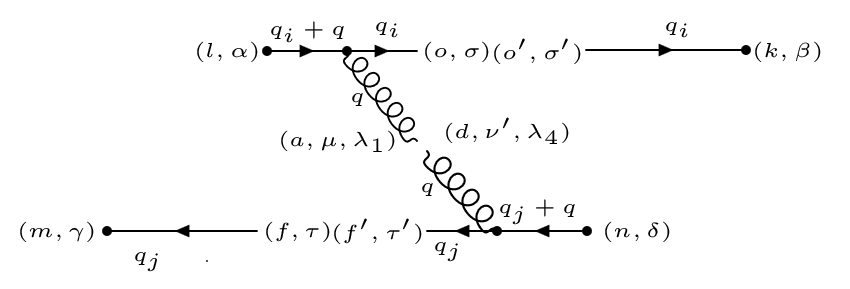
\includegraphics[width=0.85\textwidth]{images/QQ/M1M2Degaqqg.png}
\end{figure}


\begin{equation}
\begin{split}
M_1\:{\color[RGB]{255,0,0} {M_2}^{\dagger}} = [{\bar{u}}_{\sigma}(q_i)\: (-ig_s \gamma^{\mu}\times {[T^a]_o}^l) \: \frac{i(\not{q_i} + \not{q})}{(q_i + q)^2}\:\: {\varepsilon^{\lambda_1}}_{\mu} (q)] [{v}_{\tau}(q_j)]\: \\
\quad\quad\quad\quad\quad\quad\quad\quad\:\:{\color[RGB]{255,0,0}[\bar{v}_{{\tau}^{\prime}}(q_j) \: (ig_s \gamma^{{\nu}^{\prime}}\times {[T^d]_{f^{\prime}}}^n) \: \frac{-i(\not{q_j} + \not{q})}{(q_j + q)^2} \: {\varepsilon^{\lambda_4}}_{{\nu}^{\prime}} (q)]\: [{u}_{{\sigma}^{\prime}}(q_i)]}
\end{split}
\end{equation}

%Kommentar

%\begin{equation}
%\begin{split}
%M_1\: {M_2}^{\dagger} = \frac{g_s^2 {[T^a]_o}^l \:{[T^d]_{f^{\prime}}}^n }{(2q_i q)(2q_j q)} [\not{q_i}\: \gamma^{\mu} \: (\not{q_i} + \not{q})\: ]{\varepsilon^{\lambda_1}}_{\mu} (q) \: {\varepsilon^{\lambda_4}}_{{\nu}^{\prime}} (q)[\not{q_j} \:\gamma^{{\nu}^{\prime}} \: (\not{q_j} + \not{q})]\:
%\end{split}
%\end{equation}
%
%\begin{equation}
%\begin{split}
%M_1\: {M_2}^{\dagger} = \frac{g_s^2 {[T^a]_o}^l \:{[T^a]_{f^{\prime}}}^n }{(2q_i q)(2q_j q)} [\not{q_i}\: \gamma^{\mu} \: (\not{q_i} + \not{q})\: ] (-g_{{\mu}{{\nu}^{\prime}}})[\not{q_j} \:\gamma^{{\nu}^{\prime}} \: (\not{q_j} + \not{q})]\:
%\end{split}
%\end{equation}



\begin{equation}
\begin{split}
M_1\: {M_2}^{\dagger} = \frac{-g_s^2 {[T^a]_o}^l \:{[T^a]_{f^{\prime}}}^n }{(2q_i q)(2q_j q)} [\not{q_i}\: \gamma^{\mu} \: (\not{q_i} + \not{q})\: ]
\:[\not{q_j} \:\gamma_{\mu} \: (\not{q_j} + \not{q})]\:
\end{split}
\end{equation}

%Kommentar 

Expectation:
\begin{figure}[h!]
\centering
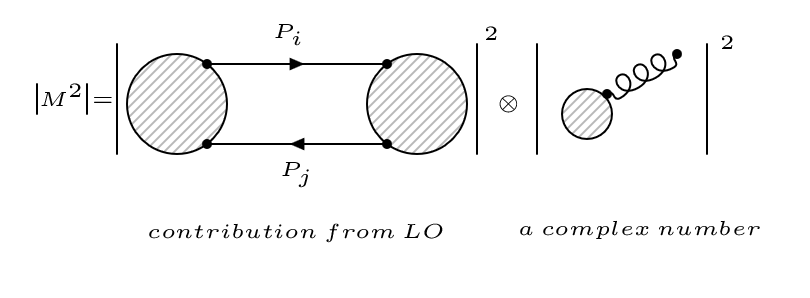
\includegraphics[width=0.85\textwidth]{images/QQ/expectationM1M2dagger.png}
\end{figure}

\begin{equation}
\begin{split}
M_1\: {M_2}^{\dagger} =& \frac{-g_s^2 {[T^a]_o}^l \:{[T^a]_{f^{\prime}}}^n }{(4(1-z)y(p_i \cdot p_j)(p_i \cdot p_j)} [(z\not{p_i} + y(1-z)\not{p_j} + \sqrt{zy(1-z)}\not{m}_{\bot})\: \gamma^{\mu} \: (\not{p_i} + y\not{p_j)}]\\
&[(1-y) \not{p_j} \:\gamma_{\mu} \: ((1-z)\not{p_i} + (1+yz-y) \not{p_j} - \sqrt{zy(1-z)}\not{m}_{\bot})]\:
\end{split}
\end{equation}

%
%\begin{equation}
%\begin{split}
%&M_1\: {M_2}^{\dagger} = \frac{-g_s^2 {[T^a]_o}^l \:{[T^a]_{f^{\prime}}}^n }{4(1-z)y(p_i \cdot p_j)(p_i \cdot p_j)} [z\not{p_i}\:\gamma^{\mu} \: \not{p_i} +zy\not{p_i}\:\gamma^{\mu}\:\not{p_j}\\
%&+y(1-z)\not{p_j}\:\gamma^{\mu} \: \not{p_i}+y^2(1-z)\not{p_j}\:\gamma^{\mu} \:\not{p_j}+\sqrt{zy(1-z)}\not{m}_{\bot}\gamma^{\mu} \: \not{p_i}\\
%&+y\sqrt{zy(1-z)}\not{m}_{\bot}\gamma^{\mu} \: \not{p_j}][(1-z) \not{p_j} \:\gamma_{\mu} \:\not{p_i}+(1+yz-y) \not{p_j} \:\gamma_{\mu} \: \not{p_j}\\
%&-(1-z)\sqrt{zy(1-z)} \not{p_j} \:\gamma_{\mu}\not{m}_{\bot}]
%\end{split}
%\end{equation}
%
%
%\begin{equation}
%\begin{split}
%&M_1\: {M_2}^{\dagger} = \frac{-g_s^2 {[T^a]_o}^l \:{[T^a]_{f^{\prime}}}^n }{4(1-z)y(p_i \cdot p_j)(p_i \cdot p_j)} [2z{p_i}^{\mu} \not{p_i} +2zy{p_i}^{\mu}\not{p_j}-zy\not{p_i}\:\not{p_j}\\
%&+2y(1-z){p_j}^{\mu} \not{p_i}-y(1-z)\not{p_j} \not{p_i}+2y^2(1-z){p_j}^{\mu}\not{p_j}+2\sqrt{zy(1-z)}{m^{\mu}}_{\bot} \not{p_i}\\
%&-\sqrt{zy(1-z)}\not{m}_{\bot} \not{p_i}+2y\sqrt{zy(1-z)}{m^{\mu}}_{\bot} \: \not{p_j}-y\sqrt{zy(1-z)}\not{m}_{\bot} \not{p_j}]\\
%&[2(1-z) {p_j}_{\mu} \not{p_i}-(1-z) \not{p_j} \not{p_i}+2(1+yz-y) {p_j}_{\mu} \not{p_j}\\
%&-2(1-z)\sqrt{zy(1-z)} {p_j}_{\mu}\not{m}_{\bot}+(1-z)\sqrt{zy(1-z)} \not{p_j} \not{m}_{\bot}]
%\end{split}
%\end{equation}
%
%
%\begin{equation}
%\begin{split}
%&M_1\: {M_2}^{\dagger} = \frac{-g_s^2 {[T^a]_o}^l \:{[T^a]_{f^{\prime}}}^n }{4(1-z)y(p_i \cdot p_j)(p_i \cdot p_j)} [4z(1+yz-y)(p_i \cdot p_j) \not{p_i} \not{p_j} \\
%&+4zy(1-z)(p_i \cdot p_j)\not{p_j}\not{p_i}+4y(1-z)^2 (p_i \cdot p_j)\not{p_j}\not{p_i}]
%\end{split}
%\end{equation}
The singular term in the denominator $ y(1-z) $ is used to drop the term with the same pre-factor and after simplification it follows:

\begin{equation}
\begin{split}
M_1\: {M_2}^{\dagger} =& \frac{-g_s^2 {[T^a]_o}^l \:{[T^a]_{f^{\prime}}}^n }{y(p_i \cdot p_j)} [\not{p_i}\not{p_j}]\times\frac{z}{1-z}
\end{split}
\end{equation}





\subsection{Final result}
\label{fin}
Because the matrix element is a complex number, there is no need to know the full interference contribution.
\begin{equation}
\lvert\:M\lvert^2\: = \lvert\:M_1\lvert^2\:+\lvert\:M_2\lvert^2\:+ M_1\: {M_2}^{\dagger} +{M_1}^{\dagger} M_2
\end{equation}
\begin{figure}[h!]
\centering
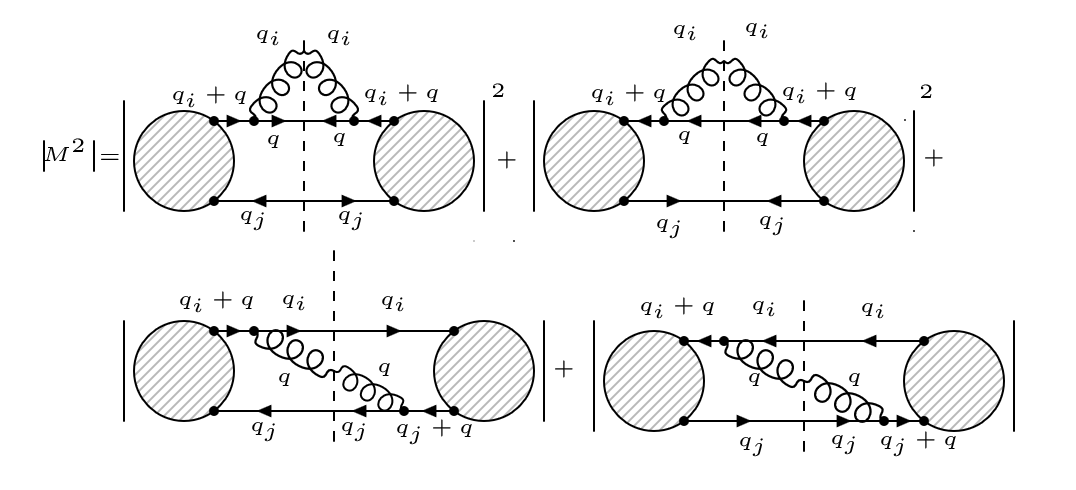
\includegraphics[width=0.85\textwidth]{images/QQ/qqgMSquer.png}
\end{figure}
Instead of $ M_1\: {M_2}^{\dagger} +{M_1}^{\dagger} M_2 $ the double of real part of $M_1\: {M_2}^{\dagger}$ will be computed.
\begin{equation}
\lvert\:M\lvert^2\: = \lvert\:M_1\lvert^2\:+\lvert\:M_2\lvert^2\:+ {\color[RGB]{255,0,0} 2RE(M_1\: {M_2}^{\dagger})}
\end{equation}
\begin{figure}[h!]
\centering
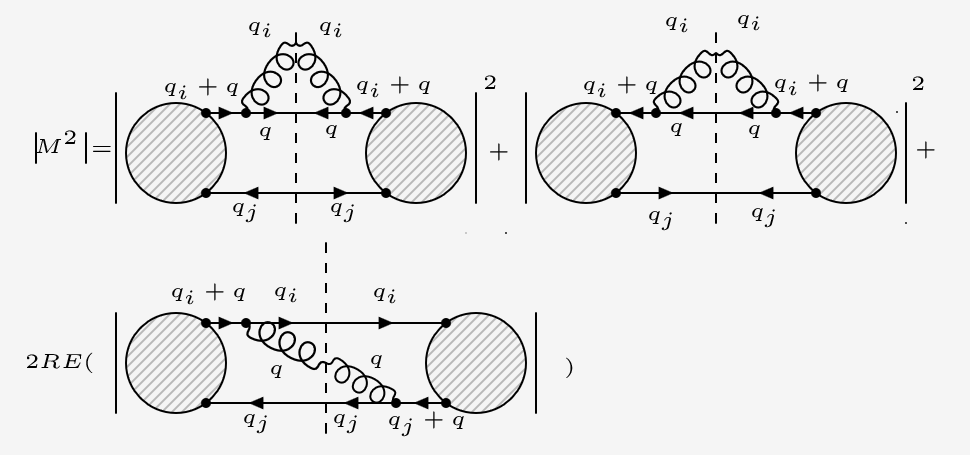
\includegraphics[width=0.85\textwidth]{images/QQ/REqqgMSquer.png}
\end{figure}
finally:
\begin{equation}
\begin{split}
&\lvert\:M\lvert^2\: = (d-2)(1-z)(1-y)\:\frac{g_s^2  {[T^a]_{o}}^k \: {[T^a]_o}^l }{2y(p_i \cdot p_j)}
[\not{p_i}][\not{p_j}]\\
&-(d-2)yz^2\:\frac{g_s^2 \: {[T^c]_f}^m \: {[T^c]_{f}}^n }{2(1-z)(1-y)(p_i \cdot p_j)}
[\not{p_i}][\not{p_j}]\\
&+2RE((\frac{-2z}{z-1}) \frac{g_s^2 \:\:{[T^a]_o}^l \:{[T^a]_{f}}^n }{2y(p_i \cdot p_j)} 
[\not{p_i}][\not{p_j}])
\end{split}
\end{equation}
The colour factors can be read from the section about the colour algebra \ref{col}. As an example, the color factor for the interference term is calculated here using the Fierz identity \ref{Fierz}:
\begin{equation}
{T^a}_{o\:k} \: {T^a}_{l\:o} = \frac{1}{2}(\delta_{oo}\delta_{lk}-\frac{1}{N}\delta_{ok}\delta_{lo})= \frac{1}{2}(N\delta_{lk}-\frac{1}{N}\delta_{lk})=C_F \delta_{lk}
\end{equation}
After summation over the final colour states and averaging over initial colour states:

\begin{equation}
{T^a}_{o\:k} \: {T^a}_{l\:o}=C_F \delta_{lk}=\frac{1}{N} \displaystyle\sum\limits_{l=1}^ N \delta_{lk}C_F=C_F
\end{equation}

The splitting function is evaluated in the case of the collinear limit:
\begin{equation}
y \longrightarrow 0
\end{equation}

%\begin{equation}
%\begin{split}
%&\lvert\:M\lvert^2\: = (d-2)(1-z)(1-y)\:\frac{g_s^2 C_F}{2y(1-2z+2z^2)(p_i \cdot p_j)}
%[\not{p_i}][\not{p_j}]\\
%&-(d-2)yz^2\:\frac{g_s^2 \: C_F }{2(1-z)(1-y)(p_i \cdot p_j)}
%[\not{p_i}][\not{p_j}]\\
%&+2RE((\frac{-2z}{z-1}) \frac{g_s^2 C_F}{2y(1-2z+2z^2)(p_i \cdot p_j)} 
%[\not{p_i}][\not{p_j}]
%\end{split}
%\end{equation}

\begin{equation}
\lvert\:M\lvert^2\: = \frac{g_s^2 C_F}{2y(1-2z+2z^2)(p_i \cdot p_j)}[\not{p_i}][\not{p_j}] \otimes((d-2)(1-z)-\frac{4z}{z-1})\:
\end{equation}
\\
for
\begin{equation}
d=4-2\epsilon
\end{equation}
%\begin{equation}
%\begin{split}
%\lvert\:M\lvert^2\: = C_F((4-2\epsilon-2)(1-z)+\frac{4z}{1-z})\:\frac{g_s^2}{2y(1-2z+2z^2)(p_i \cdot p_j)}[\not{p_i}][\not{p_j}]\\
%=C_F(\frac{2(1-\epsilon)(1-z)^2+4z}{1-z})\:\frac{g_s^2}{2y(1-2z+2z^2)(p_i \cdot p_j)}[\not{p_i}][\not{p_j}]\\
%C_F(\frac{2-4z+2z^2-\epsilon(1-z)^2+4z}{1-z})\:\frac{g_s^2}{2y(1-2z+2z^2)(p_i \cdot p_j)}[\not{p_i}][\not{p_j}]\\
%=C_F(\frac{(1+z^2)}{1-z}-\epsilon(1-z))\:\frac{g_s^2}{y(1-2z+2z^2)(p_i \cdot p_j)}[\not{p_i}][\not{p_j}]\\
%=\langle\:\hat{P_{qq}}\rangle\:\frac{g_s^2}{q_i \cdot q}[\not{p_i}][\not{p_j}]\\
%\end{split}
%\end{equation}

\begin{equation}
\begin{split}
\lvert\:M\lvert^2\: &=\frac{g_s^2}{y(p_i \cdot p_j)}[\not{p_i}][\not{p_j}]\times C_F(\frac{(1+z^2)}{1-z}-\epsilon(1-z))\\
&=\frac{g_s^2}{q_i \cdot q}[\not{p_i}][\not{p_j}]\times \langle\:\hat{P_{qq}}\rangle\:\\
\label{coll}
\end{split}
\end{equation}

With $ \langle\:\hat{P_{qq}}\rangle\: $ Alterali-Parisi splitting function \ref{Alterali-Parisi}  in the collinear limes, which was mentioned in the fifth step from the concept. This is exactly the confirmation of our calculation that our calculation was actually performed correctly, otherwise we would not have received the same splitting function for soft gluons.


\subsection{Double-check the results with the new kinematics}
With the new kinematics has to test if one gets the same result in the collinear limit. For the new parametrisation, the following substitution is used:
\begin{equation}
\begin{split}
&q_i \rightarrow q_i\\
&q \: \rightarrow k_1\\
&q_j \rightarrow q_k
\end{split}
\end{equation}
The summarized results are given here: 
\subsection*{$ |M_1|^2 $}

\begin{equation}
\begin{split}
|M_1|^2=(d-2)\:\frac{g_s^2  C_F }{(2k_1\cdot q_i)}
[\not{k_1} ][\not{q_k}]
\end{split}
\end{equation}

\begin{equation}
\begin{split}
&|M_1|^2=(d-2)\:\frac{g_s^2 \: C_F }{2y\: p_i \cdot Q}
[(\alpha_1 -y\beta_1(\frac{Q^2}{2p_i \cdot Q})) \not{p_i} + y\beta_1\not{Q} + \sqrt{y\alpha_1\beta_1}\not{n}_{\bot,1} ]\\
&[A_1\not{p_i} + A_2\not{Q} + \sqrt{1-y}\not{p_k}]
\end{split}
\end{equation}

\begin{equation}
\begin{split}
&|M_1|^2=(d-2)\:\frac{g_s^2 \: C_F }{2y\: p_i \cdot Q}
[(A_2(\alpha_1 -y\beta_1(\frac{Q^2}{2p_i \cdot Q}))+ A_1y\beta_1) {p_i}\cdot Q\\
&+(\alpha_1 -y\beta_1(\frac{Q^2}{2p_i \cdot Q}))\sqrt{1-y}p_i\cdot p_k+A_2 y\beta_1 Q^2+ \sqrt{1-y}\sqrt{y\alpha_1\beta_1}{n}_{\bot,1}\cdot p_k ]\\
\end{split}
\end{equation}

For the collinearity $ y \rightarrow 0 $ we'll get:

\begin{equation}
\begin{split}
&|M_1|^2=(d-2)\:\frac{g_s^2 \: C_F }{2y\: p_i \cdot Q}
[(A_2(\alpha_1 -y\beta_1(\frac{Q^2}{2p_i \cdot Q}))+ A_1y\beta_1) \not{p_i} \not{Q}\\
&+(\alpha_1 -y\beta_1(\frac{Q^2}{2p_i \cdot Q}))\sqrt{1-y}\not{p_i} \not{p_k}+A_2 y\beta_1 Q^2+ \sqrt{1-y}\sqrt{y\alpha_1\beta_1}\not{n}_{\bot,1} \not{p_k} ]\\
\end{split}
\end{equation}

\begin{equation}
\begin{split}
&|M_1|^2=(d-2)(1-\beta_1)\sqrt{1-y}\:\frac{g_s^2 \: C_F }{2y\: p_i \cdot Q}
[\not{p_i} \not{p_k} ]\\
\end{split}
\end{equation}

\subsection*{$ |M_2|^2 $}

\begin{equation}
\begin{split}
|M_2|^2 =(d-2) \frac{g_s^2 \: C_F }{2k_1 \cdot q_k} [\not{k_1}]\: 
[\not{q_i} ]
\end{split}
\end{equation}

\begin{equation}
\begin{split}
&|M_2|^2 =(d-2) \frac{g_s^2 \: C_F}{2k_1 \cdot q_k} [(\alpha_1 -y\beta_1(\frac{Q^2}{2p_i \cdot Q})) \not{p_i} + y\beta_1\not{Q} + \sqrt{y\alpha_1\beta_1}\not{n}_{\bot,1}]\: \\
&[(\beta_1 -\alpha_1 y(\frac{Q^2}{2p_i \cdot Q}))\not{p_i} + y\alpha_1\not{Q} - \sqrt{y\alpha_1\beta_1}\not{n}_{\bot,l} ]
\end{split}
\end{equation}

Which means:
\begin{equation}
\begin{split}
&|M_2|^2 \sim(d-2) \frac{g_s^2 \: C_F}{2k_1 \cdot q_k} y[...]\\
&\:\:\:\:\:\:\:\:|M_2|^2\rightarrow 0 \:\:\:\:\:\:\:\text{for}\:\:\:\:\: y\rightarrow 0
\end{split}
\end{equation}

\subsection*{$ M_1\: {M_2}^{\dagger} $}


\begin{equation}
\begin{split}
&M_1\: {M_2}^{\dagger} = \frac{-g_s^2\: C_F }{4y(1-\beta_1) (1-y)\:(p_i \cdot p_k)(p_i \cdot Q)} \\
&4(\beta_1 \sqrt{1-y}{p_i}\cdot {{p_k}})[\beta_1 \sqrt{1-y}\not{p_i} \not{p_k}+ (1-\beta_1) \sqrt{1-y}\not{p_i}\not{p_k}]
\end{split}
\end{equation}

\begin{equation}
\begin{split}
&M_1\: {M_2}^{\dagger} = \frac{-g_s^2\: C_F }{y(1-\beta_1) \:(p_i \cdot p_k)(p_i \cdot Q)} \beta_1( {p_i}\cdot {{p_k}})[\beta_1 \not{p_i} \not{p_k}+ (1-\beta_1) \not{p_i}\not{p_k}]
\end{split}
\end{equation}

\begin{equation}
\begin{split}
&M_1\: {M_2}^{\dagger} = \frac{\beta_1}{(1-\beta_1)} \times \: \frac{-g_s^2\: C_F }{y \:(p_i \cdot Q)} [\not{p_i} \not{p_k}]
\end{split}
\end{equation}

With the transformation $ \beta_1 \rightarrow z $, the same results are obtained in each step and hence, it was demonstrated that with the new kinematics the same splitting function can be obtained as in the old parametrisation.
